% !TeX encoding = UTF-8
% !TeX program = pdflatex
% !TeX spellcheck = en_US

\documentclass[LaM,binding=0.6cm]{./packages/sapthesis/sapthesis}

\usepackage{microtype}
\usepackage{amssymb}
\usepackage{amsmath}
% Norm Command
\newcommand{\norm}[1]{\left\lVert#1\right\rVert}

\usepackage{hyperref}
\hypersetup{pdftitle={Robustness of Deep Neural Networks Using Trainable Activation Functions},pdfauthor={Federico Peconi}}

% Remove in a normal thesis
\usepackage{lipsum}
\usepackage{curve2e}
\definecolor{gray}{gray}{0.4}
\newcommand{\bs}{\textbackslash}

% Commands for the titlepage
\title{Robustness Of Deep Neural Networks \\Using Trainable Activation Functions}
\author{Federico Peconi}
\IDnumber{1823570}
\course{Computer Science}
\courseorganizer{Computer Science - Informatica LM-18}
\AcademicYear{2019/2020}
\copyyear{2020}
\advisor{Prof. Simone Scardapane}
%\advisor{Dr. Nome Cognome}
%\coadvisor{Dr. Nome Cognome}
\authoremail{peconi.1823570@studenti.uniroma1.it}

\examdate{Something October 2020}
\examiner{Prof. Nome Cognome}
\examiner{Prof. Nome Cognome}
\examiner{Dr. Nome Cognome}
\versiondate{\today}



\begin{document}

\frontmatter

\maketitle
\dedication{Dedicated to\\ Donald Knuth}

\begin{abstract}
This document is an example which shows the main features of
the \LaTeXe\ class \texttt{sapthesis.cls} developed by 
with the help of GuIT (Gruppo Utilizzatori Italiani di \TeX).
\end{abstract}

\begin{acknowledgments}
Ho deciso di scrivere i ringraziamenti in italiano
per dimostrare la mia gratitudine verso i membri
del GuIT, il Gruppo Utilizzatori Italiani di \TeX, e, in particolare,
verso il prof. Enrico Gregorio.
\end{acknowledgments}

\tableofcontents

% Do not use the starred version of the chapter command!
%\chapter{Capitolo non numerato}





\mainmatter

\chapter{Introduction}

    \section{Intriguing Properties of Neural Networks}

        Here we informally state the problem of adversarial attacks in ML models 
        especially wrt to Neural Networks.
        Why is it of fundamental importance for the progress of the field from
        both practical (nns cant yet be deployable in critical scenarios for such reasons ) 
        and theoretical (Madry arguments around interpertability and robustness)
        perspectives

    \section{Smooth Activation Functions and Robustness}

        Recently a link has been proposed between activation functions and the robustness of
        Neural Networks (Smooth Adversarial Training). In particular, authors showed how they managed
        to improve the robustness by replacing the traditional Rectified Linear Units activation functions
        with smoother alternatives such as ELUs, SWISH, PReLUs
        
        Building up from this result we thought we could find benefits by laveraging recently proposed smooth
        trainable activation functions called Kernel Based Activation Functions (Scardapane et al.), 
        which already showed great results in standard tasks, in the context of adversarial attacks.
        
    \section{Structure of the Thesis}

        Description of the remaining chapters 


\chapter{Fundamentals}

    In this chapter, the basic concepts needed to understand the main arguments for the thesis are introduced. Pointers to more appropriate and detailed resources on the topics are given throughout

    \section{Deep Neural Networks}
        
        Broadly speaking, the field of Machine Learning is the summa of any algorithmic methodology whose aim is to automatically find meaningful patterns inside data without
        being explicitly programmed on how to do it. Well known examples are: Search Trees (ref.), Support Vector Machines (ref. ), Clustering (ref.) and, more recently, 
        Neural Networks (ref. ). During the last two decades Neural Networks gained a lot of attention for their outstanding performances in different tasks like
        image classification (ref. ImageNet, over human level), speech and audio processing(ref ).

        \subsection{Definition}
            
            Neural Networks (NNs) are often used in the context of Supervised Learning where the objective is to model a parametric function 
            $ f_{\theta} \colon \mathcal{X} \to \mathcal{Y}$ given $n$ input-output pairs $S = \{(\mathbf{x_i}, y_i)_{i=1}^n\} $ with $\mathbf{x_i} \in \mathcal{X}$ and $ y_i \in \mathcal{Y}$
            such that
            \[
                f_{\theta} \sim f  
            \]
            where $f$ is assumed to be the real input-output distribution that we want to learn. In plain words, this means that we want to find the best set of parameters $\theta^{*}$ for the model
            such that, for any unseen input $x_{new}$ we have that $f_{\theta^*}\left(x_{new}\right)$ is as close as possible to $f\left(x_{new}\right)$

            For the sake of explanation, assume the input, which in practice can be very complex and unstructured e.g. made of: graphs, text, sounds, ecc, to be embedded in an input space  $\mathcal{X} = \mathbb{R}{^d}$.
            The simplest form of a neural network is then given by
            \[
                f_{W, b}\left(x\right) = \sigma(Wx + b)
            \]
            where the parameters of the network are the elements of a $u \times d$ matrix $ W $ and a $u$-dimensional vector called bias. The last element applied at the end is the $ \sigma $ 
            function which consists of a non-linear function acting element-wise and is the key component to introduce non linearity in NNs allowing them to model 
            highly non-linear functions. We call it \textit{activation function}.
            \[
                f_{W, b}\left(x\right) = \left[\sigma(W_1^{\intercal} x + b_1), \sigma(W_2^{\intercal} x + b_2), \ldots, \sigma(W_u^{\intercal} x + b_u)\right]
            \]
            Where $W_i$ and $b_i$ are respectively the i-th row of $W$ and the i-th element of the bias.
            
            Historically, the whole picture was somehow biologically inspired and had an intuitive explanation. Indeed, if we think at $ W $ as weights i.e. $ w_{ij} $ as the importance
            the model gives to the input $x_i$ for how much it contributes to the $ f_{W}\left(x\right)_j $-th component and define $ \sigma $ to be
            \begin{equation}
                \label{step}
                \sigma(W_j^{\intercal} x + b_j) = \begin{cases} 
                    1 & W_j^{\intercal}x \geq - b_j \\
                    0 & W_j^{\intercal}x < - b_j 
                \end{cases}  
            \end{equation}
            then it is easy to see that here the bias is acting like a threshold which discrminates between \textit{activating} or not the $j$-th component depending on how much importance was given. 
            Due to this analogy with the behaviour of neurons in the brain we call each component \textit{neuron}, non-linearities activation functions and the whole model neural network.
            \begin{figure}[h]
                \centering
                \includegraphics[width=0.5\textwidth]{slide1}
                \caption{Graphic representation of a one layer NN also know as MLP(ref. )}
            \end{figure}
            \paragraph{}
            In general, the idea of a layer of neurons can be recursively extended by stacking more layers together, all of which are described by a matrix of weights, a bias and an activation function
            and letting the output of one becoming the input of the subsequent.
            The resulting model is the mathematical composition of the layers, thus if we let $ L $ be the number of layers, $ z_0 = \mathbf{x} $ and $ z_l = \sigma_l\left(W_{l}z_{l-1} + b_l\right)$
            we write a $L$-layered $f_{\mathbf{W}, \mathbf{b}}$:
            \[
                f_{\mathbf{W}, \mathbf{b}} = z_L = \sigma_{L}\left(W_{L}\sigma_{L-1}\left(\ldots\left(W_2\sigma_{1}\left(W_{1}z_{0} +b_1\right)+ b_2\right)\ldots\right)+ b_{L}\right)
            \]
            With $ \mathbf{W} = \{W_1, \ldots, W_{L}\} $ and $ \mathbf{b}= \{b_1, \ldots, b_{L}\} $. We will call the first layer \textit{input layer}, the middle layers \textit{hidden layers}
            and the last layer \textit{output layer}.
            \begin{figure}[h]
                \centering
                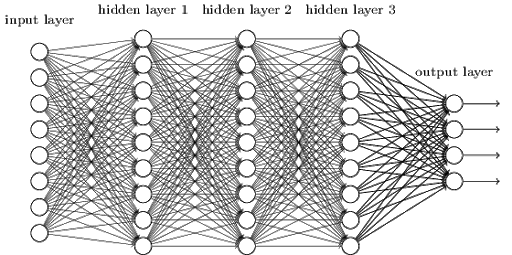
\includegraphics[scale=0.5]{fnn}
                \caption{A Feedforward Neural Network with 3 hidden layers(ref. Michael A. Nielsen, Neural Networks and Deep Learning, Determination Press', 2015)}
                \label{fig:fnn}
            \end{figure}
            This general but still basic form of Neural Network is known as \textit{Feed Forward Neural Network} Fig. \ref{fig:fnn}. 
        \subsection{Training}

            There are still a couple of important pieces left to define to develop a properly working Neural Network. For instance, how are parameters computed? And in particular, with respect to what we compute them? 
            \subsubsection{Loss Function}
                Before we realized that our goal is to maximize the approximation of the ground-truth input-output relation that lies under the data, therefore there is a need to
                introduce some metric to quantify this approximization. Call \textit{loss function} $ L(f_{\theta}\left(x\right), y) \colon \mathcal{Y} \times \mathcal{Y} \to \mathbb{R_+}$ 
                such metric. Common choices are (ref.):
                \begin{itemize}
                    \item Least Square: $\norm{f_{\theta}\left(x\right) - y}^2$ for regression tasks 
                    \item Binary Cross-Entropy: $y \log (f_{\theta}(x))+(1-y) \log (1-f_{\theta}(x))$ for binary classification  
                    \item Categorical Loss Function: $-\sum_{c=1}^{C} y_{c} \log \left(f_{\theta}(x)_c\right)$ for mulicategory classification with $C$ classes.
                \end{itemize}
                Intuitively, a good loss function will map bad approximations to high values and good approximations to smaller ones.
                Nevertheless, those are only point-wise estimates of the error, hence the best empirical solution learnable from the training set $ S $ would be 
                \begin{equation}
                    \label{erm}
                    \displaystyle{  \min_{\theta}  \frac{1}{n} \sum_{i=1}^{n} L\left(f_{\theta}\left(x_{i}\right), y_{i}\right) }
                \end{equation}
                which is called \textit{empirical risk minimization}.
            \subsubsection{Gradient Descent}
               So far we have described, given an input $ \mathbf{x} $, how we can compute the output of a feedforward neural network by means of compositions of dot products 
               and non-linear transformations between matrices, starting from the first to the very last of the layers in what is called a \textit{forward pass}. As it turns out, to attempt to solve \ref{erm} we need to follow the exact
               opposite path. Indeed, every optimization algorithm used in practice makes use of the same subroutine called Backpropagation (ref.  ) introduced in the 1970s, which allows to compute, starting from the output layer
               and going backwards, the partial derivative of the loss function with respect to each weight in the network. Moreover it does so efficiently requiring only one \textit{backward pass}.

               Let $i^l = W_l z_{l-1} + b_l$ be the weighted input to the $l$-th layer, then the key observation is that the only way $ W_l $ can affect the loss function is by affecting linearly
               the next layer which in turn affects its next layer and so on. In particular assume we add a little change $\Delta i_{j}^{l} $ to the $j$-th 
               element of $ i^l $ so that the neuron will output $ \sigma \left(i_{j}^{l} + \Delta i_{j}^{l}\right) $, this change will
               eventually propagates in the network causing the overall loss $LS$ to change by an amount $\frac{\partial LS}{\partial i_{j}^{l}} \Delta i_{j}^{l}$. For brevity,
               denote the gradient of the weighted input on the j-th neuron $ \delta^{l}_{j} = \frac{\partial LS}{\partial i^{l}_{j}} $, then the following holds:
               \begin{equation}
                 \delta^{L}_{j} = \frac{\partial LS}{\partial i^{L}_{j}} = \frac{\partial LS}{\partial z^{L}_{j}}\frac{\partial z^{L}_{j}}{\partial i^{L}_{j}} \\
                                =\frac{\partial LS}{\partial z^{L}_{j}} \sigma_{L}^{\prime}(i^{L}_{j})
               \end{equation}
               and equally, taking into account the whole output layer
               \begin{equation}
                    \label{bp1}
                    \delta^{L}=\nabla_{z^L} LS \odot \sigma^{\prime}(i^{L})
               \end{equation}
               where $ \odot $ is the element-wise product and $ \nabla_{x} $ the vector of the partial derivatives $ \partial LS / \partial x $. 
               That is, the gradient with respect to the weighted input to the last layer is given, using the chain rule, by the gradient with respect to the activation of the last layer times the derivative
               of the last activation function. Similarly, for any hidden layer $ l $ we note that:
               \begin{equation}
                \label{bp2}
                    \delta^{l}=\left((W^{l+1})^{T} \delta^{l+1}\right) \odot \sigma^{\prime}(i^{l})
                \end{equation}
                When we apply the transpose weight matrix, $(W^{l+1})^{T}$, think intuitively of this as moving the previous layer's gradient backward, giving a measure of the gradient at the output of the $l$-th layer. 
                We then take the product $\sigma^{\prime}(i^{l})$ which again moves the gradient backward through the activation function in layer $l$, giving the gradient of the weighted input to layer $l$.

                By combining \ref{bp1} with \ref{bp2} we can compute the gradient $\delta^{l}$ for any layer in the network. We start by using \ref{bp1} to compute on the last layer, 
                then apply equation \ref{bp2} to compute $\delta^{L-1}$, then the same equation again to compute $\delta^{L-2}$, and so forth, 
                all the way back until the input layer. Since our intent is to retrieve the gradients for every weights of the network, we are left to 
                show how $ \delta^l $ relates to them, here we provide such relation without giving an explicit proof which instead can be found in many
                texts like (ref Nielsen chapter 2).
                \begin{equation}
                    \frac{\partial LS}{\partial b^{l}_{j}} = \delta^{l}_{j}
                \end{equation}
                \begin{equation}
                    \frac{\partial LS}{\partial w^{l}_{i,j}} = z^{l-1}_i \delta^{l}_{j}.
                \end{equation}
                Remark how we already know how to compute each element on the right sides of these equations, moreover, given that the activation function
                and its derivative is efficiently computable, we will be able to efficiently get the seeked gradients in just one pass.
                It is worth mention that Backpropagation is actually a special case of a more generic set of programming techniques that go under
                the name of \textit{Automatic Differentiation} (Ref. ) to numerically evaluate the derivative of a function specified by a computer program.
                Such techniques are usually implemented in modern numerical libraries building variations of a data structure called \textit{computational graph}.
                Well known examples are \textit{Autograd} in \textit{Pytorch} (Ref. ) or \textit{GradientTape} in \textit{TensorFlow} (Ref. ).

               What does it mean to be able to compute partial derivatives of the loss? It means being able to understand where and how 
               the loss decreases and thus we can exploit such information to find better and better weights solutions. 
               This is the idea behind the Gradient Descent algorithm (Ref. ). In particular, the gradient of a weight is nothing but the
               direction inside the weight-space where the loss function is increasing, therefore what we want to do is to follow the opposite
               direction. Formally, this translates in the following weight update rules:
               \begin{equation}
                    w^{t}_{l} \rightarrow w_{l}^{t+1}=w^{t}_{l}-\frac{\eta}{n} \sum_{j} \frac{\partial LS_{\mathbf{x}_{j}}}{\partial w^{t}_{l}}
               \end{equation}
               \begin{equation}
                b^{t}_{l} \rightarrow b^{t+1}_{l}=b^{t}_{l}-\frac{\eta}{n} \sum_{j} \frac{\partial LS_{\mathbf{x}_{j}}}{\partial b^{t}_{l}}
               \end{equation}

            where $w_{l}^{t}$ are the values of the weights for layer $l$-th during the $t$-th pass, $\eta$ is a small positive constant called \textit{learning rate}
            chosen by the user accordingly and the gradients are averaged among all samples in the training set. 
            \begin{figure}[h!]
                \centering
                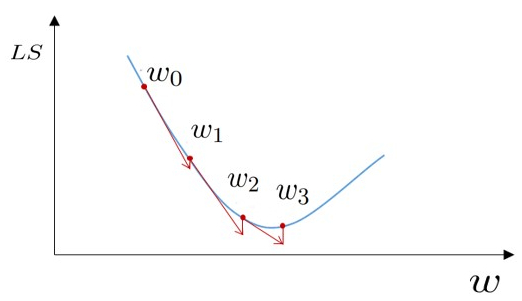
\includegraphics[scale=0.5]{gd}
                \caption{A 1-D representation of 4 gradient descent steps}
                \label{fig:gd}
            \end{figure}
            Most importantly, note how we take the negative of the gradients, meaning that we are following the direction in which the loss decreases Fig. \ref{fig:gd}. The distance
            between two consecutives weights $\Delta_{w^t}$ well be directly proportional to both the learning rate picked and the averaged gradient.

            In practice, however, when very often we are deling with thousands or milions of data points, becomes unfeasable to compute every pass over
            the entire training set, thus what is done is to split the data into so called \textit{mini-batches} and then apply the
            update rules on each mini-batch until we scanned the whole data. The entire scan is called \textit{epoch} and the 
            resulting algorithm Stochastic Gradient Descent (Ref. ). Lastly, the size of a mini-batch is another hyperparameter 
            that should be tuned by the developer, keeping in mind that the bigger the size the more stable will be our training
            the smaller the size the faster the training.

            \begin{figure}[h]
                \centering
                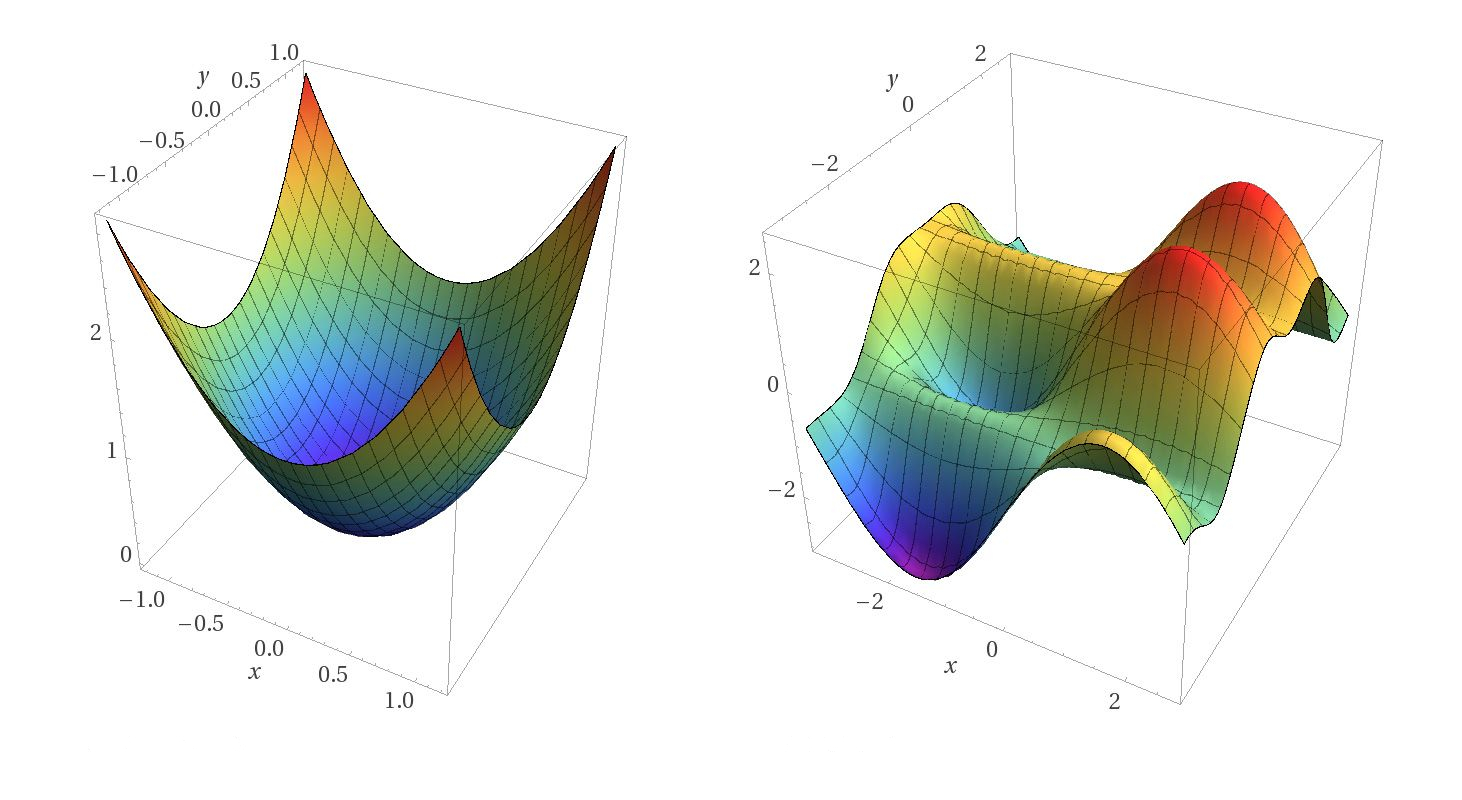
\includegraphics[scale=0.25]{conv_nonconv}
                \caption{Convex and Non-convex optimization landscapes}
                \label{fig:convnonconv}
            \end{figure}
            As stated earlier, neural networks can model extremely non-convex input-output functions therefore in principle there
            is no guarantee that Gradient Descent will find the optimal solution to \ref{erm} Fig. \ref{fig:convnonconv}.
            Indeed, the optimal solution would be the global minimum of our weighted loss function but there is no apparent
            way for the algorithm to distinguish between global, local minimum or saddle points Fig. \ref{fig:globlocsad}.
            However, it turns out that in practice Gradient Descent works fairly well once we correctly tune
            hyperparameters and run the algorithm from different initial values. (Ref .)
            Moreoever, lately authors have been proposed different methods to improve the convergence and the efficiency by 
            smart changes of the learning rate during the training process (ref . cyclical learning rates) 
            \begin{figure}[h]
                \centering
                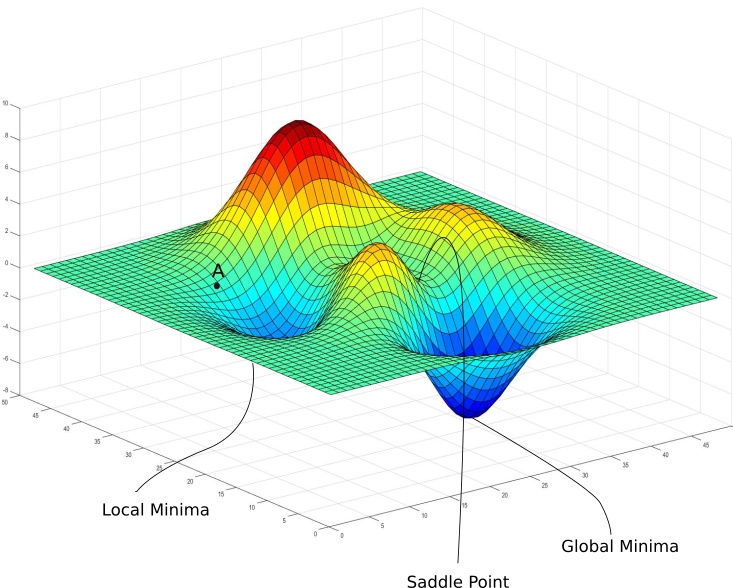
\includegraphics[scale=0.35]{globlocsad}
                \caption{Visualization of global, local and saddle points. How can A reach the global minimum?}
                \label{fig:globlocsad}
            \end{figure}

        \subsection{Activation Functions}
            
            We have seen how the learning process works optimizing the empirical risk by means of gradients computation.
            Therefore to be able to optimize anything, a neural network needs to have only differentiable components.
            However, before in \ref{step} we discussed the so called \textit{step function}, an activation function that, 
            even if biologically inspired and easier to justify, is not differentiable at the origin and the derivative is 0 elsewhere.
            Thus if we think again about how Backpropagation works, we see that employing such activation function would make the weight updates impossible
            since already $ \delta^{L} $ would be either undefined or 0.

            To deal with this issue, one of the first proposed activation functions was an approximation of the step function known as \textit{sigmoid} (Ref. ) 
            \begin{equation}
                \textnormal{sigmoid}(x) = \frac{1}{1 + e^{-x}}
            \end{equation}
            which is differentiable everywhere with continuous derivatives (property that we will refer as \textit{smoothness} through the chapters) and
            maps to $ [0, 1] $ values.
            \begin{figure}[h]
                \centering
                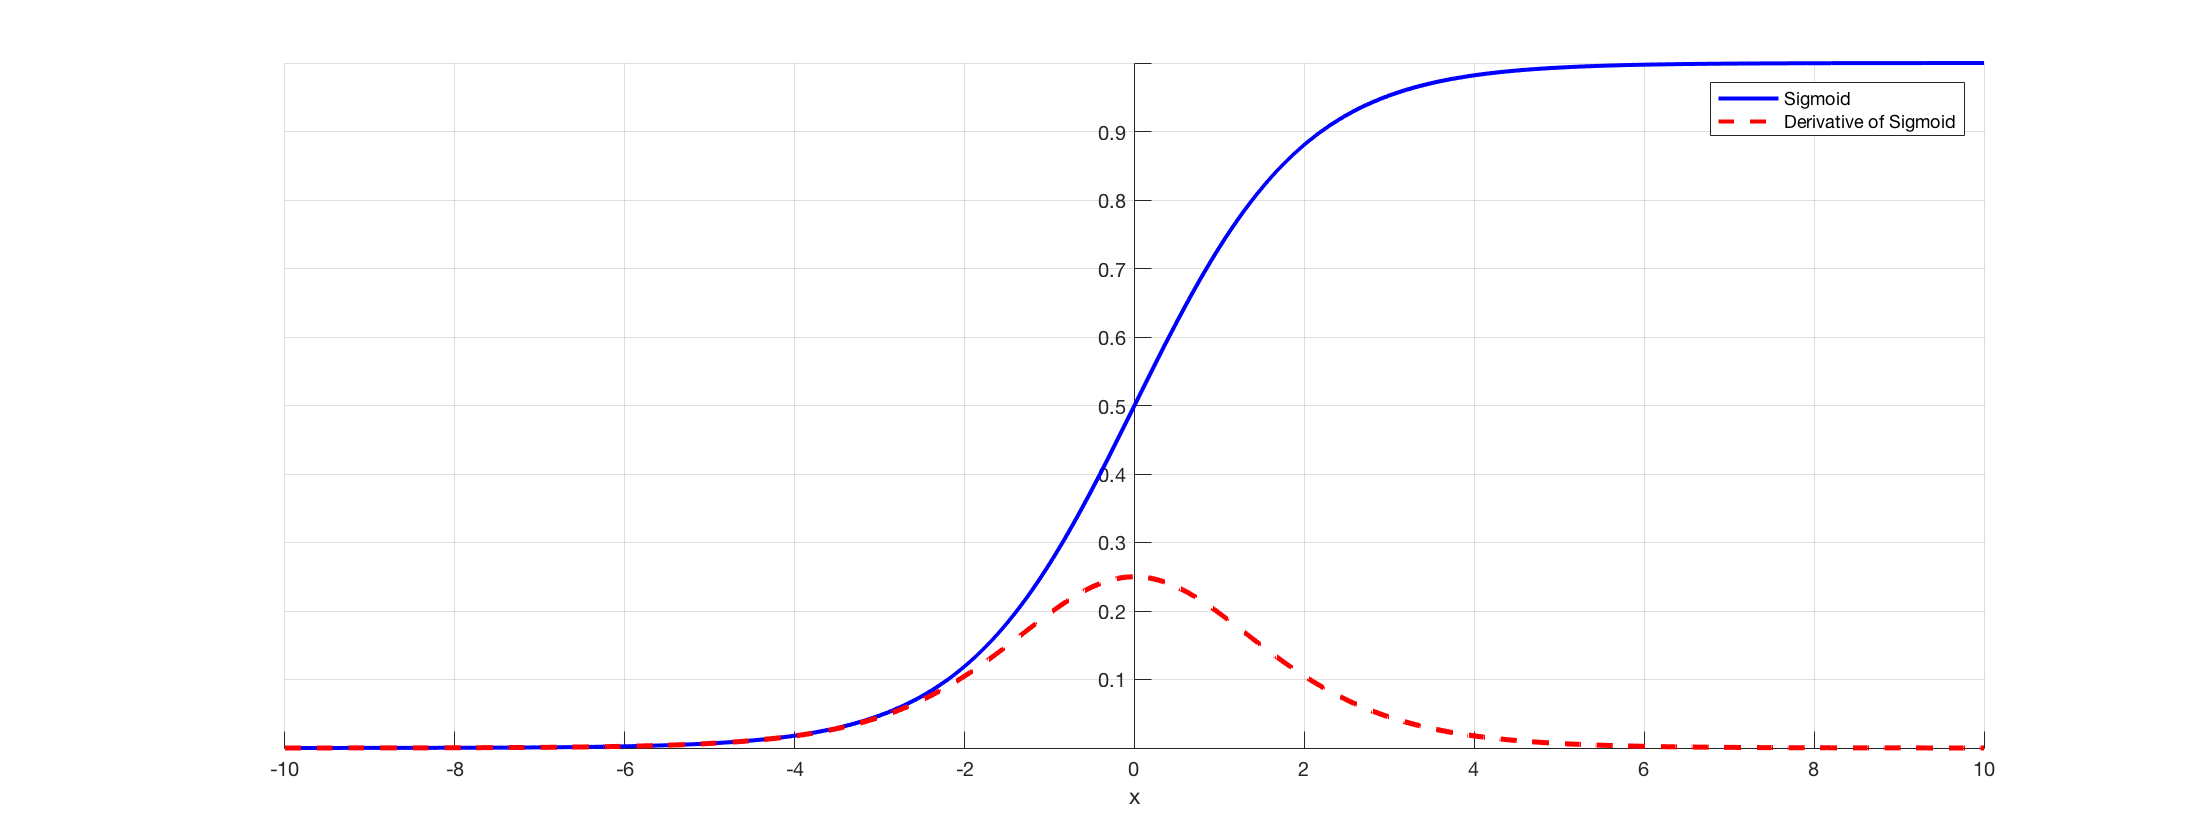
\includegraphics[width=1\textwidth]{sig_der}
                \caption{Plot of the Sigmoid function and its first derivative.}
                \label{fig:sigmoid}
            \end{figure}
            Nevertheless, as the number of layers increases and the network becomes sufficiently deep, the sigmoid suffers from the \textit{vanishing gradient} problem (Ref. ) Fig. \ref{fig:sigmoid}
            due to its derivative being $[0, 0.25]$ bounded. Mainly for this reason it is not widely adopted in practice.

            More in general, the sigmoid lies inside a class of activation functions known as \textit{squashing} i.e. monotonically non-decreasing functions $\varSigma$
            that satisfy
            \begin{equation}
                \lim_{x \to - \infty} \sigma(x) = c, \quad 
                \lim_{x \to \infty} \sigma(x) = 1.
            \end{equation}
            For example, another kind of activation function of this type is the \textit{hyperbolic tangent}, defined as
            \begin{equation}
                \tanh (x)=\frac{\exp \{x\}-\exp \{-x\}}{\exp \{x\}+\exp \{-x\}},
            \end{equation}
            which was find to allow for universal expressivness of nets (Ref. ). However, as for the sigmoid, squashing functions tend to be prone to vanishing 
            and exploding gradients (Ref. ).

            Nowadays, the most used activation function in neural networks for different applications is the \textit{rectifier linear unit} (ReLU),
            first introduced in (Ref. Hahnloser et al. in 2000) and defined as the positive part of its argument
            \begin{equation}
                \textnormal{ReLU}(x) = \max(0, x),
            \end{equation}
            allows for efficient training and alleviates the exploding gradient problem (having derivative either 0 or 1), introducing only one point of
            non-differentiability. Moreover, it promotes \textit{sparsness} in the network, which is usually beneficial (Ref. ). One problem with ReLUs though 
            is that the neuron's value, that get pushed to a big negative number, might stay stucked in 0 for essentially all inputs, in a so called \textit{dead state}.
            If many neurons in the network die this can afflict the model capacity and can be seen as a form of vanishing gradient problem. To overcome this problem,
            a slighlty different activation functions can be used, called \textit{leaky ReLU} (Ref. ):
            \begin{equation}
                \operatorname{Leaky ReLU}(x)=\left\{\begin{array}{ll}
                    x & \text { if } x \geq 0 \\
                    \alpha x & \text { otherwise },
                    \end{array}\right.
            \end{equation}
            where $\alpha > 0$ is a user-defined constant usually set to small values such as 0.01. Even if this solutions solves the dying neurons problem, it does
            affect the sparseness property of ReLUs.
            
            By definition, the mean of ouput values from a ReLU is always positive. \textit{Exponential linear unit} (ELU) try to normalize their inputs:
            \begin{equation}
                \operatorname{ELU}(x)\left\{\begin{array}{ll}
                    x & \text { if } x \geq 0 \\
                    \alpha(\exp \{x\}-1) & \text { otherwise },
                    \end{array}\right.
            \end{equation}
            saturating negative values at a user-defined value $- \alpha$ which is usually set to 1. Conversly to ReLU and LeakyReLUs, the derivative is continuous
            therefore the function is smooth and for the negative values is defined as $ELU(x) + \alpha$.

            Finally, one more recent activation function which gained a lot of attention is the \textit{Swish} function (Ref. ):
            \begin{equation}
                \operatorname{swish}(x)= \operatorname{sigmoid}(x) * x,
            \end{equation}
            
            \begin{figure}[hb!]
                \centering
                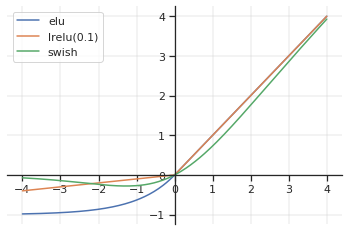
\includegraphics[scale=0.50]{afunctions}
                \caption{ELU, LeakyReLU($\alpha=0.1$) and Swish functions plotted together. It can be seen that they mostly differ for negative values whereas behaving very similar to ReLU for positive arguments.}
                \label{fig:afuncs}
            \end{figure}
            which again does look like another approximation of a ReLU Fig. \ref{fig:afuncs}, but in this case it manages in not loosing any useful property. Indeed, since
            it also saturates at 0 for negative values, it allows for sparsity and being smooth around 0 it helps reducing dying neurons. Lastly, around 0 negative 
            values are kind of preserved which may still be relevant to patterns in the underlying data.
            Swish function proved to consistently match if not outperform ReLU networks in different domains (Ref. ), and more recent studies showed how this function
            can also help in training more \textit{robust} networks (Ref. Smooth Adversarial training).

            Along with this list of more 'traditional' activation functions, which we will call \textit{fixed} activation functions, there is a whole branch of
            more sophisticated solutions, where the idea is to \textit{learn} the function's optimal shape employing suitable parametric functions. 
            Such functions can then be trained together with other weights of the net using backpropagation and gradient descent. Moreover, following the terminology
            introduced in (Ref Scardapane t al KafNets) we can again distinguish between two classes of this learnable activation functions: the so called
            \textit{parametric activation functions} and \textit{Non-parametric activation functions}. The former being usually a parametrization of a fixed 
            activation function involving few constant parameters, whereas the latter is called non-parametric due to the number of parameters that can in principle
            grow without a bound and involves more complex shapes. At the end of this chapter we introduce a recently proposed class of non-parameteric activation functions,
            called \textit{Kernel-Based Activation Functions} which will then be the main tool used in the following chapters to try to build more robust neural networks.    


        \subsection{CNNs: Convolutional Neural Networks}

            In computer vision, in particular for image processing tasks, we can make the assumption that the input to the model will be an image. 
            How well do feedforward neural networks adapt to such inputs? It turns out that we need to introduce several changes in the architecture to expect 
            them to work properly. Take for example the famous dataset \textit{ImageNet} which consists of more than $ 14 $ milions of images,
            all of which made of $ 256 \times 256 \times 3 $ pixels. Every fully connected neuron would have $ 256 * 256 * 3 =  196608 $ weights, thus for a neural network
            with $ 1000 $ of such neurons, which is a very small number of units in practice, we would already need to train almost $ 200 $ milions of parameters,
            which requires a lot of resources. Therefore feedforward neural networks do not scale well to bigger images. More importantly, assume our task is to 
            classify an image, from the point of view of such models, if we take an image $x$ and translate it to the lets say right for few pixels, with high 
            probability it will look like a completly different image from the point of view of the net and will probably be classified differently, even if 
            from our point of view is clearly the same image. In some sense, there is no apparent way in which fully connected neural networks can take advantage of 
            concepts such as \textit{locality} or \textit{translation invariance} that are intrinsic to images.
            
            To circumvent these limitations, reasearchers have developed a specific architecture targeted for computer vision tasks called \textit{Convolutional Neural Network} (CNN) (Ref. ).
            In a standard CNN, every layer is $3$-dimensional $(Width \times Height \times Dept) $ to reflect the fact that we are always dealing with images 
            and each neuron is connected only to a constant number of nearby neurons in the previous layer, shrinking down the number of total weights required.
            Layers can be either \textit{convolutive layers} or \textit{pooling layers} or \textit{fully-connected layers}, the latter being a normal hidden layer.

            A convolutive layer takes in input $W \times H \times C_{in}$ neurons from the previous layer and outputs $W \times H \times C_{out}$ neurons, where $ C_{out}$
            is the number of filters used by the layer. A filter $F$ is a $K \times K \times C_{in}$ matrix of trainable weights, with $K>0$ typically a small integer, which is used to
            compute a 2-dimensional activation map by sliding (convolving) across the width and height of the input. At each slice of input 
            $ \mathbf{x_{ij}} = (x^{1}_{ij}, x^{2}_{ij}, \ldots, x^{C_{in}}_{ij})$ that it touches, it computes the dot product $ F^{T}X_{ij}$
            where $X_{ij}$ is the $K \times K \times C_{in}$ window centered at $\mathbf{x_{ij}}$. Visually:
            \begin{figure}[hb!]
                \centering
                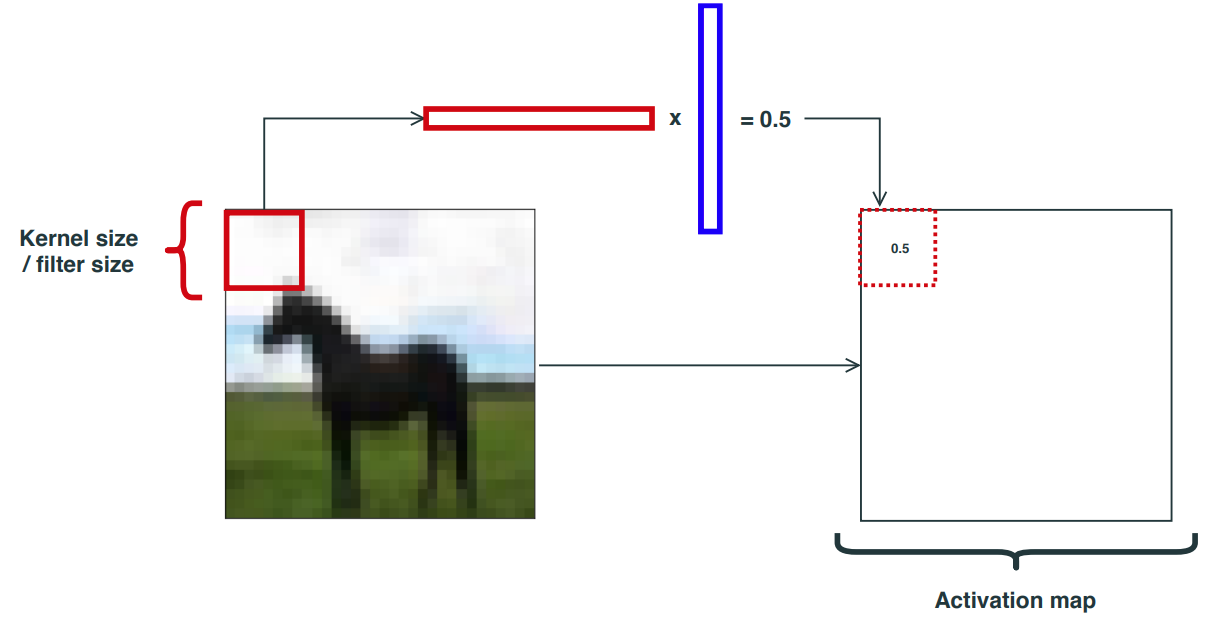
\includegraphics[scale=0.30]{convolution}
                \caption{A convolution that produces the first element of the activation map for the given filter.}
                \label{fig:conv}
            \end{figure}
            Intuitively, through backpropagation we learn filters tha are capable of recognizing specific shapes in the image, which we can see as features,
            starting from very concise ones in the early layers to more global ones towards the end layers as the receptive field gets larger(Ref. ). 
            Typically, as for normal neural networks, we apply a non-linear transformation after each convolutive layer and by stacking many of these Convolutional
            layers we get a convolutional network.
            
            Going deeper in the network as we learn global features, it might be convenient to reduce the width and the heigh dimensions, for this reason CNNs employ pooling layers
            that filters the inputs by some metric, such as average or max values.  



        \subsection{From Neural Networks to Deep Neural Networks}
        

    \section{Adversarial Examples Theory}

        Formal definition of what is an adversarial attacks plus currently well known attacks

    \section{Defenses}

        Review of the literature on defenses to improve robustness: provable robustness, adversarial training

    \section{Kernel Based Activation Functions}


\chapter{Related Works}

    \section{K-Winners Take All}
    \section{Smooth Adversarial Training}


\chapter{Solution Approach}
 
    Comparing the activations's distributions for different activation functions (ReLU, KWTA, Kafs) 
    seem to suggest Kafs might be good candidates to improve model robustness 

    \section{Lipschitz Constant Approach}

        On the limitations of current Lipischitz-Constant based approaches especially when involving Kafs

    \section{Fast is Better than Free Adversarial Training}

        Adversarial training (Madry et al.) and current methods to improve the efficiency (Fast is better than free)


\chapter{Evaluation}

    \section{VGG Inspired Architectures Results}

    \section{Explofing Gradients with KafNets}

        The exploding gradients problem with KafResNet, why is it happening? (still to clarify)

    \section{ResNet20 Inspired Architectures Results}


\chapter{Future Works}

    Different Kernels, resolve the exploding gradient problem and scale to ImageNet
    Perform more adaptive attacks to assess the robustness of kafresnets as is the current standard (Carlini et al.)


\chapter{Conclusions}

    This thesis tries to add to the bag of evidences in literature that smoother architectures might benefit improvements in adversarial resiliency
    
    
\appendix


\backmatter
% bibliography
%\cleardoublepage
%\phantomsection
%\bibliographystyle{sapthesis} % BibTeX style
%\bibliography{bibliography} % BibTeX database without .bib extension

\end{document}
